\documentclass[conference]{IEEEtran}
\IEEEoverridecommandlockouts
\usepackage{cite}
\usepackage{amsmath,amssymb,amsfonts}
\usepackage{algorithmic}
\usepackage{graphicx}
\usepackage{textcomp}
\usepackage{xcolor}
\usepackage{booktabs}
% figur bersama kedua track ada di paper/figures/; TEXINPUTS tidak dipakai
% graphicx, jadi jalur relatifnya harus disebut eksplisit di sini.
\graphicspath{{figures/}{../figures/}}
\def\BibTeX{{\rm B\kern-.05em{\sc i\kern-.025em b}\kern-.08em
    T\kern-.1667em\lower.7ex\hbox{E}\kern-.125emX}}

% ---------------------------------------------------------------------------
% CATATAN DRAF -- HARUS DIMATIKAN SEBELUM SUBMIT.
% Ganti \draftnotestrue menjadi \draftnotesfalse; seluruh penanda merah hilang
% dalam satu langkah. Jangan menghapusnya satu per satu.
%
% Status refs.bib per 19 Agustus 2026: hanya berisi satu citekey yang relevan
% (prabhavalkarHybridPETCTRadiomics2026). Entri lain adalah sisa Zotero yang
% tidak berhubungan. Setiap \CITE di bawah menandai klaim yang membutuhkan
% sitasi dan belum punya kuncinya. Jangan mengarang citekey: kalau kuncinya
% belum ada di refs.bib, penanda tetap dibiarkan sampai ekspor Zotero berikutnya.
% ---------------------------------------------------------------------------
\newif\ifdraftnotes
\draftnotestrue
\newcommand{\CITE}[1]{\ifdraftnotes\textcolor{red}{\,[SITASI: #1]}\fi}

\begin{document}

\title{Radiomics-CNN Fusion and Per-Arm Explainability for Lung Nodule Malignancy Classification on LIDC-IDRI}

\author{\IEEEauthorblockN{1\textsuperscript{st} Habb}
\IEEEauthorblockA{\textit{Department of ...} \\
\textit{University}\\
City, Country \\
email@domain.com}
\and
\IEEEauthorblockN{2\textsuperscript{nd} Kolaborator}
\IEEEauthorblockA{\textit{Department of ...} \\
\textit{University}\\
City, Country \\
email@domain.com}
}

\maketitle

\begin{abstract}
Fusing handcrafted radiomics with convolutional neural network (CNN) features is a common strategy for lung nodule malignancy classification, but its benefit over either modality alone is usually reported as a single accuracy number, without separating how much of that number depends on checkpoint selection and without asking what the fused model can explain that its parts cannot. We evaluate a decision-level fusion arm that averages CNN and radiomics probabilities against both single-modality arms on LIDC-IDRI, using a patient-level five-fold split and pooled DeLong tests, and we repeat every comparison under two checkpoint regimes: the epoch selected by validation AUC, and the unselected end-of-training epoch. Late fusion significantly outperforms the CNN-only arm on all three backbones under both regimes ($p<10^{-9}$ across both regimes; $p<10^{-11}$ under the unselected regime alone). Against the radiomics-only arm we do not rest a parity claim on a non-significant DeLong test, which would be an inference from absence of evidence; we test equivalence directly, with two one-sided tests against a margin of 0.02 AUC fixed on clinical grounds before the analysis. Equivalence holds on all three backbones under both checkpoint regimes ($p_\text{TOST}<0.004$), including the two cases where DeLong does reject equality of the AUCs under the unselected regime: those differences are statistically detectable and clinically negligible at the same time. The same test refuses equivalence against CNN-only on all six comparisons, as it must. On explainability, late fusion inherits the image branch unchanged, so its class-activation maps differ from the CNN-only maps only on nodules where the two arms disagree; pointing accuracy differs by at most 0.05 and is identical on a fixed six-nodule display set. Late fusion is therefore the only arm that supplies spatial and feature-level evidence simultaneously, at no measurable cost in localization quality and none in AUC.
\end{abstract}

\begin{IEEEkeywords}
lung nodule malignancy, radiomics, decision-level fusion, explainable AI, Grad-CAM, SHAP, LIDC-IDRI
\end{IEEEkeywords}

\section{Introduction}
Computer-aided diagnosis of pulmonary nodule malignancy from CT increasingly combines two complementary sources of evidence: handcrafted radiomics features that quantify shape, texture, and intensity statistics of a segmented nodule, and deep convolutional features learned end-to-end from image patches. The premise of fusion is that the two sources capture non-redundant information and that combining them should match or exceed either alone. This premise does not always hold on cohorts of the size available for lung nodule malignancy prediction, where radiomics with feature selection is a strong baseline in its own right \cite{prabhavalkarHybridPETCTRadiomics2026}.

We argue that reporting fusion as a single AUC obscures two questions a reviewer will ask. First, how much of the reported margin survives when the checkpoint-selection advantage is removed? A CNN arm whose epoch is chosen by AUC on the very fold later used for reporting carries an advantage that a gradient-boosted radiomics model fitted without a validation set does not, so any comparison between them is weighed on an uneven scale unless the regime is stated. Second, if fusion only matches a single modality on accuracy, what does it actually buy? We answer the second question in the currency of explainability rather than accuracy: the fused arm is the only one that can produce both a spatial saliency map and a feature-level attribution for the same prediction.

This paper contributes: (1) a decision-level fusion arm evaluated against both single-modality arms with pooled DeLong tests across five disjoint folds, and, for the parity claim specifically, a formal equivalence test against a margin fixed in advance rather than an appeal to a non-significant $p$-value; (2) a checkpoint-regime sensitivity analysis that reports every comparison twice, under the selected and the unselected checkpoint, and shows that the equivalence conclusion is regime-independent although the significance conclusion is not; and (3) a quantitative comparison of explanation quality between the late-fusion and CNN-only arms, which measures rather than assumes what the added modality does to localization, together with an architectural account of why the effect is confined to the nodules on which the two arms disagree.

\section{Related Work}
Radiomics-based malignancy prediction on LIDC-IDRI-scale cohorts routinely reaches AUC in the 0.79 to 0.94 range and is frequently competitive with or superior to end-to-end deep learning under the same sample size.\CITE{2--3 studi radiomics LIDC-IDRI dengan rentang AUC yang dikutip} Fusion of a weaker modality with a stronger one has been documented to degrade rather than improve joint performance, a phenomenon attributed to modality competition during joint training, in which the dominant modality dictates the gradient signal and the joint representation collapses toward it.\CITE{modality competition / greedy multimodal learning} Decision-level fusion sidesteps that failure mode by construction, since no joint representation is learned and neither branch can dominate the other's gradients; the price is that the fused model has no capacity to discover cross-modal interactions.\CITE{taksonomi early/intermediate/late fusion} Gated and attention-based fusion mechanisms occupy the middle ground, letting a network learn how much to weight each modality rather than fixing that weight in advance.\CITE{Gated Multimodal Unit}

The finding that fusion fails to beat handcrafted radiomics by a meaningful margin is not peculiar to this study. A comparative study on a LIDC-derived cohort of comparable size reports tuned conventional radiomics at AUC 0.921, end-to-end deep learning at 0.824, and a hybrid model at 0.938: the hybrid's advantage over radiomics alone is 0.017 AUC, the same order as the gaps reported here, and the authors describe the tuned conventional and deep-feature models as comparable rather than ranked.\CITE{Astaraki et al. 2021, Frontiers in Oncology} Reviews across other anatomies reach the same conclusion, finding deep learning only slightly superior to handcrafted radiomics and the comparison inconsistent across clinical applications.\CITE{systematic review radiomics vs deep learning} The literature is genuinely split rather than settled: several fusion studies do report clear gains over single modalities.\CITE{2--3 studi fusi yang melaporkan keunggulan} What is consistent is that in the one-to-two-thousand-sample regime the gain, when present, is small.

Arguing for a model on the strength of what it can explain, rather than what it scores, also has precedent. The normative case for preferring interpretable models in high-stakes decisions is made directly in the literature,\CITE{Rudin 2019, Nature Machine Intelligence} and two LIDC-specific models have been justified on the same basis: a hierarchical semantic CNN whose malignancy AUC of 0.856 barely exceeds a black-box 3D CNN at 0.847, and a capsule model predicting radiologist-defined visual attributes at accuracy on par with black-box counterparts.\CITE{HSCNN, Shen et al. 2019} \CITE{X-Caps, LaLonde et al. MICCAI 2020} We are not aware of a study that compares explanation quality across fusion arms on lung nodules, which is the specific gap this paper addresses, within the limits stated in Section~\ref{sec:limits}.

\section{Methods}

\subsection{Dataset and split}
We use LIDC-IDRI.\CITE{Armato et al., makalah dataset LIDC-IDRI} Nodules are aggregated per patient and assigned malignancy labels from the median of four expert ratings on a 1 to 5 scale,\CITE{konvensi agregasi label median LIDC} collapsed to benign (rating below 3), malignant (rating above 3), and indeterminate (rating equal to 3, excluded from the binary arm). The dataset is partitioned into five folds by patient identifier, seeded at 42, so that no patient contributes cases to more than one fold. All backbones and all arms train and evaluate on the identical fold assignment. After the join between the image cohort and the radiomics feature table, which drops nodules with duplicate \texttt{(patient\_id, nodule\_idx)} keys, 1366 nodules remain; every number in this paper is computed on that common cohort, so no two arms are compared on different denominators.

\subsection{Preprocessing}
Each nodule is represented as a 2.5D patch: a stack of adjacent axial slices centered on the nodule, resampled and cropped to a fixed in-plane resolution. Hounsfield unit intensities are clipped to $[-1000, 400]$ and rescaled to $[0, 1]$.

\subsection{Backbones and input resolution}
The fusion analysis uses three backbones that reached the highest standalone localization quality in a preceding seven-backbone screen: ConvNeXt-Tiny\CITE{ConvNeXt}, DenseNet201, and DenseNet121\CITE{DenseNet}. The backbone set is fixed in advance and is not searched over. All backbones are evaluated at a uniform upsampled input of 96 pixels, the smallest multiple of 32 above the minimum input size demanded by any backbone in the wider screen, so that no backbone receives a resolution advantage that would confound the explainability comparison.

\subsection{Representation arms}
Five arms are defined per backbone and fold. \emph{CNN-only} is the backbone's own classification head. \emph{Radiomics-only} is a gradient-boosted classifier\CITE{XGBoost} trained on the handcrafted radiomics feature vector\CITE{PyRadiomics / IBSI} after per-fold selection, in which a mutual-information filter (\texttt{mutual\_info\_classif}) retains the 50 highest-scoring candidates and LASSO with cross-validated regularization performs the final selection, both fitted on the training fold alone. \emph{Early fusion} concatenates the CNN embedding with the selected radiomics vector into a single feature matrix and trains a gradient-boosted classifier on it. \emph{Intermediate fusion} projects the CNN embedding and the radiomics vector into learned subspaces and concatenates them before a shared classification head trained end-to-end. \emph{Late fusion}, the arm under test in this paper, averages the two arms' malignancy probabilities,
\begin{equation}
p_\text{late} = 0.5 \, p_\text{CNN} + 0.5 \, p_\text{radiomics},
\label{eq:late}
\end{equation}
and adds no trained parameters. Fig.~\ref{fig:arch} shows all five arms and marks late fusion as the arm this paper measures. We deliberately do not search over fusion architectures: the object of study is what a fixed, minimal fusion rule buys, not which of many rules scores highest on this cohort.

\subsection{Checkpoint regimes}
Every AUC and every DeLong test is computed twice. The \emph{selected} regime loads the epoch chosen by validation AUC on the same fold that is later reported. The \emph{unselected} regime loads the final training epoch, which carries no selection advantage. The radiomics-only arm is fitted without any validation set and is therefore identical under both regimes; it is the only arm whose number does not move, which is precisely why it is the comparison the regime affects. The unselected regime is a lower-bound sensitivity check, not a nested cross-validation. A nested inner split is in fact used for the parameterised intermediate-fusion arm, which is trained in its own stage; it cannot be extended to the arms reported here without retraining all three backbones over all five folds, because the CNN probabilities consumed by both the CNN-only and late-fusion arms come from backbone checkpoints frozen upstream of the fusion stage.

\subsection{Statistical protocol}
Probabilities from the five disjoint validation folds are concatenated into a single vector per arm, from which one AUC and one DeLong test\CITE{DeLong et al. 1988} per arm pair are computed. Pooling rather than averaging per-fold statistics keeps every nodule in the test exactly once and avoids combining correlated per-fold $p$-values.

A DeLong test that fails to reject cannot establish that two arms are equivalent: its null is equality, and not rejecting a null is not evidence for it.\CITE{Lakens 2017, equivalence testing primer} Every claim of parity in this paper is therefore made with a separate test whose null is the opposite one. We apply two one-sided tests to the paired AUC difference,\CITE{Liu, Ma, Wu \& Tai 2006, paired-AUC equivalence} rejecting the composite null that the difference is at least as large as an equivalence margin $\delta$ in either direction. Equivalence is declared at $\alpha=0.05$ when both one-sided tests reject, which is the same statement as the 90\% confidence interval on the difference lying entirely inside $\pm\delta$. The standard error is the DeLong variance of the difference, so the equivalence test and the significance test read the same quantity and cannot disagree about the data.

We set $\delta = 0.02$ AUC. The margin is fixed on clinical grounds before any equivalence test is run, and it is not revised afterwards. Two considerations set it. First, malignancy rating on this dataset is itself unreliable at a scale far exceeding 0.02: the four LIDC readers disagree substantially on the malignancy characteristic,\CITE{Lin et al. 2017, interobserver disagreement LIDC} so a model difference below that noise floor cannot change a management decision that the reference standard itself does not determine. Second, reported performance on LIDC moves by more than 0.02 AUC in response to sample-selection and label-truthing choices alone,\CITE{Baltatzis et al. 2021, pitfalls of sample selection} which means a difference of that size is not stable enough to act on. The value is also conservative relative to the 0.05 and 0.10 margins commonly debated for non-inferiority in diagnostic accuracy studies; we prefer the tighter margin because a loose one makes equivalence easy to declare and correspondingly uninformative.

\subsection{Explainability protocol}
For the image branch, Layer-CAM maps\CITE{Layer-CAM; Grad-CAM sebagai pendahulunya} are computed at the backbone's deepest convolutional stage and evaluated with dice overlap, IoU, a size-matched dice variant, a pointing-game hit rate\CITE{pointing game, Zhang et al.}, and an energy-based pointing metric\CITE{energy-based pointing game, Score-CAM}, all against the radiologist-annotated nodule mask. A class-activation map explains one decision class; for the CNN-only arm that class is $\arg\max p_\text{CNN}$, and for late fusion it is $\arg\max p_\text{late}$. On nodules where the two arms predict the same class the two maps are identical by construction, since (\ref{eq:late}) leaves the image branch untouched. We therefore report, alongside every metric, the number of nodules on which the two arms disagree, so a zero difference can never be misread as a measurement that was not performed. Metrics are reported on two sample sets: a fixed six-nodule display set frozen before this analysis and never reselected, and the 60-nodule fold-0 set used by the earlier explainability stage, which gives finer resolution than a six-sample pointing rate can. For the radiomics branch, SHAP values\CITE{Lundberg \& Lee 2017; TreeSHAP} quantify the contribution of each handcrafted feature. The two explanation modalities are reported separately rather than combined into a single score, because no model-agnostic metric currently allows a fair joint comparison between a spatial map and a tabular attribution.

\begin{figure}[htbp]
\centerline{
\includegraphics[width=\columnwidth]{fusion_architecture.png}}
\caption{The five representation arms. Late fusion, highlighted, combines the branches only at the probability level and adds no trained parameters; the remaining four arms are the tested comparators.}
\label{fig:arch}
\end{figure}

\section{Results}

\subsection{Combined advantage}
Table~\ref{tab:combined} summarizes what each arm delivers, in accuracy and in explanation, on the same cohort and the same folds. Ranges in parentheses span the three backbones.

\begin{table}[htbp]
\caption{What each arm delivers, pooled over 5 folds; ranges span 3 backbones}
\begin{center}
\footnotesize
\begin{tabular}{p{1.85cm}p{1.6cm}p{1.6cm}p{1.6cm}}
\toprule
\textbf{Criterion} & \textbf{CNN-only} & \textbf{Radiomics-only} & \textbf{Late fusion} \\
\midrule
AUC, selected checkpoint & 0.8944 (0.8907--0.8965) & 0.9336 & 0.9327 (0.9300--0.9363) \\
AUC, unselected checkpoint & 0.8806 (0.8725--0.8888) & 0.9336 (unaffected) & 0.9290 (0.9241--0.9360) \\
DeLong vs.\ late fusion, selected & significant 3/3 & significant 0/3 & --- \\
Equivalent to late fusion within 0.02 AUC & no, 0/6 & yes, 6/6 & --- \\
Spatial saliency map & yes & structurally impossible & yes (inherited) \\
Pointing accuracy, 60 nodules & 0.6667 (0.5763--0.7288) & undefined & 0.6384 (0.5593--0.6780) \\
Radiomic feature SHAP & no & yes & yes \\
\textbf{Spatial and feature evidence together} & \textbf{no} & \textbf{no} & \textbf{yes} \\
\bottomrule
\end{tabular}
\label{tab:combined}
\end{center}
\end{table}

\subsection{Late fusion versus CNN-only: unconditional}
Late fusion significantly outperforms the CNN-only arm on every backbone under both checkpoint regimes (Table~\ref{tab:delong}). The $p$-values are no larger under the unselected regime than under the selected one; the largest value across all six tests is $1.4\times10^{-10}$, so $p<10^{-9}$ is the bound covering both regimes, and $p<10^{-11}$ holds if only the unselected regime is quoted.

This comparison is structurally immune to the checkpoint-selection confound described in Section~\ref{sec:limits}: both arms load the same CNN checkpoint, so whatever advantage selection confers enters both sides of the test and cancels. Only the comparison against radiomics-only is regime-sensitive, because radiomics-only is the one arm that never had a validation set to select on.

\begin{table}[htbp]
\caption{Pooled DeLong tests, late fusion versus each single-modality arm}
\begin{center}
\footnotesize
\begin{tabular}{llcc}
\toprule
\textbf{Backbone} & \textbf{Comparison} & \textbf{Selected} & \textbf{Unselected} \\
\midrule
ConvNeXt-Tiny & vs.\ CNN-only  & $1.0\times10^{-12}$ & $3.9\times10^{-12}$ \\
DenseNet201   & vs.\ CNN-only  & $1.4\times10^{-10}$ & $7.4\times10^{-12}$ \\
DenseNet121   & vs.\ CNN-only  & $3.0\times10^{-11}$ & $3.8\times10^{-15}$ \\
\midrule
ConvNeXt-Tiny & vs.\ radiomics & 0.4555 & \textbf{0.0246} \\
DenseNet201   & vs.\ radiomics & 0.4901 & 0.5122 \\
DenseNet121   & vs.\ radiomics & 0.6793 & \textbf{0.0144} \\
\bottomrule
\end{tabular}
\label{tab:delong}
\end{center}
\end{table}

\subsection{Equivalence with radiomics}
The DeLong tests against radiomics-only in Table~\ref{tab:delong} tell two different stories depending on the regime. Under the selected checkpoint none of the three backbones differs significantly from radiomics-only. Under the unselected checkpoint, ConvNeXt-Tiny and DenseNet121 do differ, and in the unfavourable direction ($p=0.0246$ and $p=0.0144$); only DenseNet201 is non-significant under both. Read as a parity claim, that would make parity a property of two of six comparisons, and would make it depend on a checkpoint choice that has nothing to do with the radiomics branch.

Table~\ref{tab:tost} shows that this reading is an artefact of asking the wrong question. Equivalence within the pre-specified margin of 0.02 AUC holds on all three backbones under both regimes, with $p_\text{TOST}$ between $8\times10^{-7}$ and $3.7\times10^{-3}$ and every 90\% interval contained in $\pm 0.02$. The largest difference anywhere in the six comparisons is 0.0095 AUC, on DenseNet121 under the unselected checkpoint, whose interval reaches $-0.0160$ at its far end and still stops short of the margin. The two comparisons DeLong flags are therefore both true statements at once: the difference is large enough to be detected on 1366 nodules, and too small to matter. This is the expected behaviour of a significance test at this sample size and not a contradiction between the two tests, which share the same variance estimate.

The negative control confirms the test discriminates. Applied to late fusion against CNN-only, where the differences run from 0.035 to 0.052 AUC, the same procedure refuses equivalence on all six comparisons ($p_\text{TOST}>0.99$). Fig.~\ref{fig:fig16} plots all twelve intervals against the margin band.

Non-inferiority, the one-sided form of the same test, holds on all twelve comparisons: late fusion is never worse than either single-modality arm by 0.02 AUC or more.

We retain DenseNet201 as the primary model, now on a narrower ground than before: it is the backbone on which the stronger claim of statistical indistinguishability also survives both regimes, and it is the only one whose point estimate favours fusion under both. The equivalence claim itself does not depend on that choice. The magnitude of the selection advantage is small in absolute terms, at most 0.0078 AUC, and it reverses no arm ordering.

\begin{table}[htbp]
\caption{Equivalence tests against radiomics-only, margin $\delta=0.02$ AUC. $\Delta$ is late fusion minus radiomics-only; the interval is the 90\% confidence interval on $\Delta$. All six are equivalent; none is merely non-significant}
\begin{center}
\footnotesize
\begin{tabular}{llccc}
\toprule
\textbf{Backbone} & \textbf{Regime} & $\Delta$ & \textbf{90\% CI} & $p_\text{TOST}$ \\
\midrule
ConvNeXt-Tiny & selected   & $-0.0036$ & $(-0.0115,\ 0.0043)$ & $3.3\times10^{-4}$ \\
ConvNeXt-Tiny & unselected & $-0.0068$ & $(-0.0117, -0.0018)$ & $5.7\times10^{-6}$ \\
DenseNet201   & selected   & $+0.0027$ & $(-0.0037,\ 0.0090)$ & $3.6\times10^{-6}$ \\
DenseNet201   & unselected & $+0.0024$ & $(-0.0036,\ 0.0084)$ & $8.2\times10^{-7}$ \\
DenseNet121   & selected   & $-0.0017$ & $(-0.0085,\ 0.0051)$ & $4.4\times10^{-6}$ \\
DenseNet121   & unselected & $-0.0095$ & $(-0.0160, -0.0031)$ & $3.7\times10^{-3}$ \\
\bottomrule
\end{tabular}
\label{tab:tost}
\end{center}
\end{table}

\begin{figure}[htbp]
\centerline{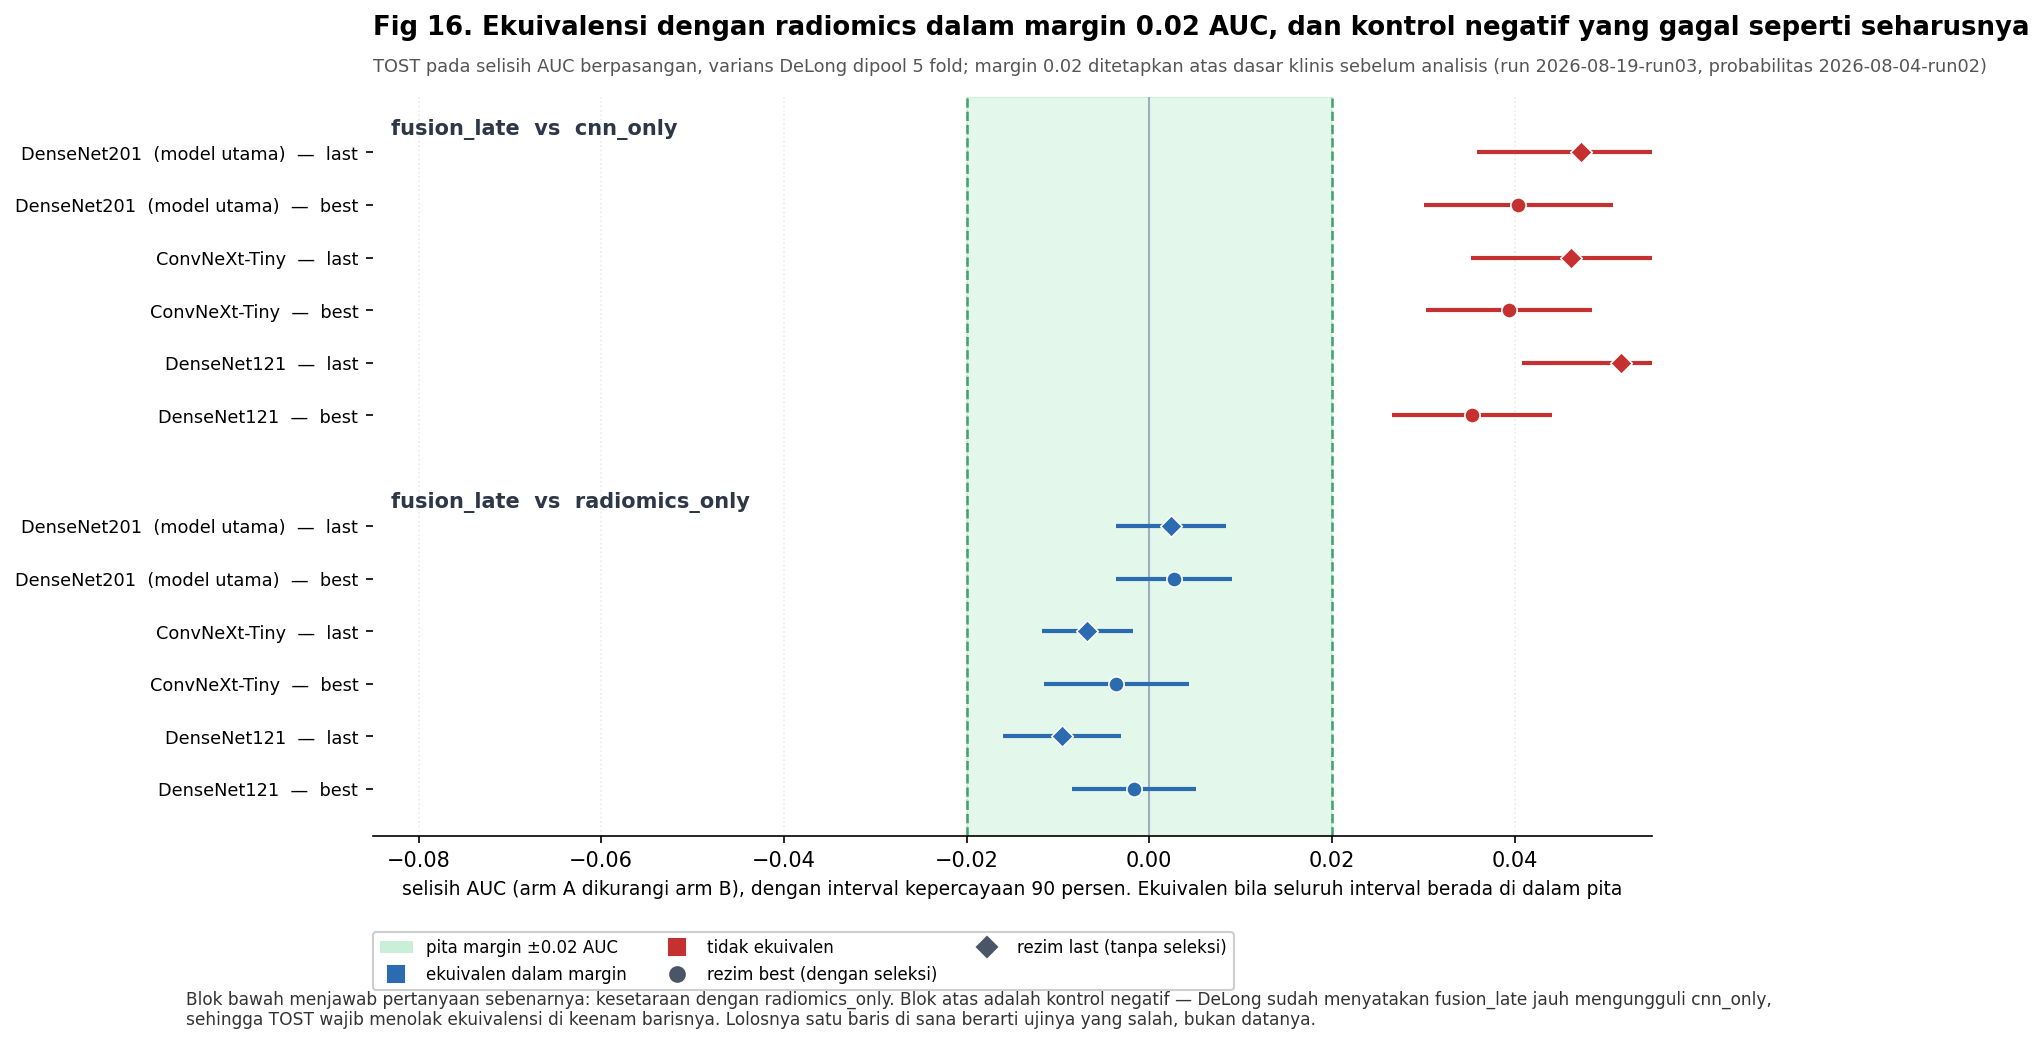
\includegraphics[width=\columnwidth]{fig16_tost_equivalence.png}}
\caption{All twelve equivalence tests. Every interval against radiomics-only lies inside the $\pm0.02$ margin band; every interval against CNN-only lies outside it, which is the negative control the test has to fail.}
\label{fig:fig16}
\end{figure}

\subsection{Explainability}
Table~\ref{tab:xai} reports pointing accuracy for the CNN-only and late-fusion arms on both sample sets. On the fixed six-nodule set the two arms are identical to the last digit, because the arms agree on the predicted class for all six nodules. On the 60-nodule set they differ by at most 0.0508, and the number of disagreeing nodules is 5, 6, and 2 out of 59.

\begin{table}[htbp]
\caption{Pointing accuracy, CNN-only versus late fusion. $n_{\ne}$ is the number of nodules on which the two arms predict different classes}
\begin{center}
\footnotesize
\begin{tabular}{llccc}
\toprule
\textbf{Backbone} & \textbf{Set} & \textbf{CNN-only} & \textbf{Late fusion} & $n_{\ne}$ \\
\midrule
ConvNeXt-Tiny & fixed 6    & 1.0000 & 1.0000 & 0 \\
DenseNet201   & fixed 6    & 0.3333 & 0.3333 & 0 \\
DenseNet121   & fixed 6    & 0.5000 & 0.5000 & 0 \\
\midrule
ConvNeXt-Tiny & 60 nodules & 0.7288 & 0.6780 & 5 \\
DenseNet201   & 60 nodules & 0.6949 & 0.6780 & 6 \\
DenseNet121   & 60 nodules & 0.5763 & 0.5593 & 2 \\
\bottomrule
\end{tabular}
\label{tab:xai}
\end{center}
\end{table}

The reading the numbers support is that adding a radiomics modality does not damage the image branch's localization. It is not that fusion explains better: late fusion's pointing accuracy is nominally at or below CNN-only's everywhere, and we claim no explainability advantage in the localization metrics.

We state plainly what the spatial channel of the fused arm is, because the alternative would be to let a reader infer more than the construction supports. Late fusion's class-activation map is the CNN branch's map. There is no fused network to explain: (\ref{eq:late}) combines two scalars, so the only model a saliency method can attach to is the image branch itself, and the map is recomputed on that same backbone with only the explained class possibly differing. Nothing in the spatial channel is novel to the fused arm, and the near-zero differences in Table~\ref{tab:xai} are a consequence of that fact rather than an empirical discovery about fusion. The corollary is the useful half: a decision-level rule acquires a spatial explanation at no cost, because it never trains a joint representation that could distort one. Parameterised fusion has no such guarantee, and we do not test it here.

What late fusion adds is a second, non-substitutable kind of evidence. Fig.~\ref{fig:fig14} shows both for the same model and fold: a spatial map answering where the evidence lies, and a SHAP summary answering which handcrafted features drove the decision. The CNN-only arm has no counterpart to the second panel, and the first panel is structurally impossible for radiomics-only, which never sees an image.

The SHAP panel is presented once rather than once per backbone. The radiomics branch of the late-fusion arm receives no input from the CNN, so its SHAP summary is identical across backbones by construction; publishing three copies of the same plot would imply a per-backbone variation that does not exist.

\begin{figure}[htbp]
\centerline{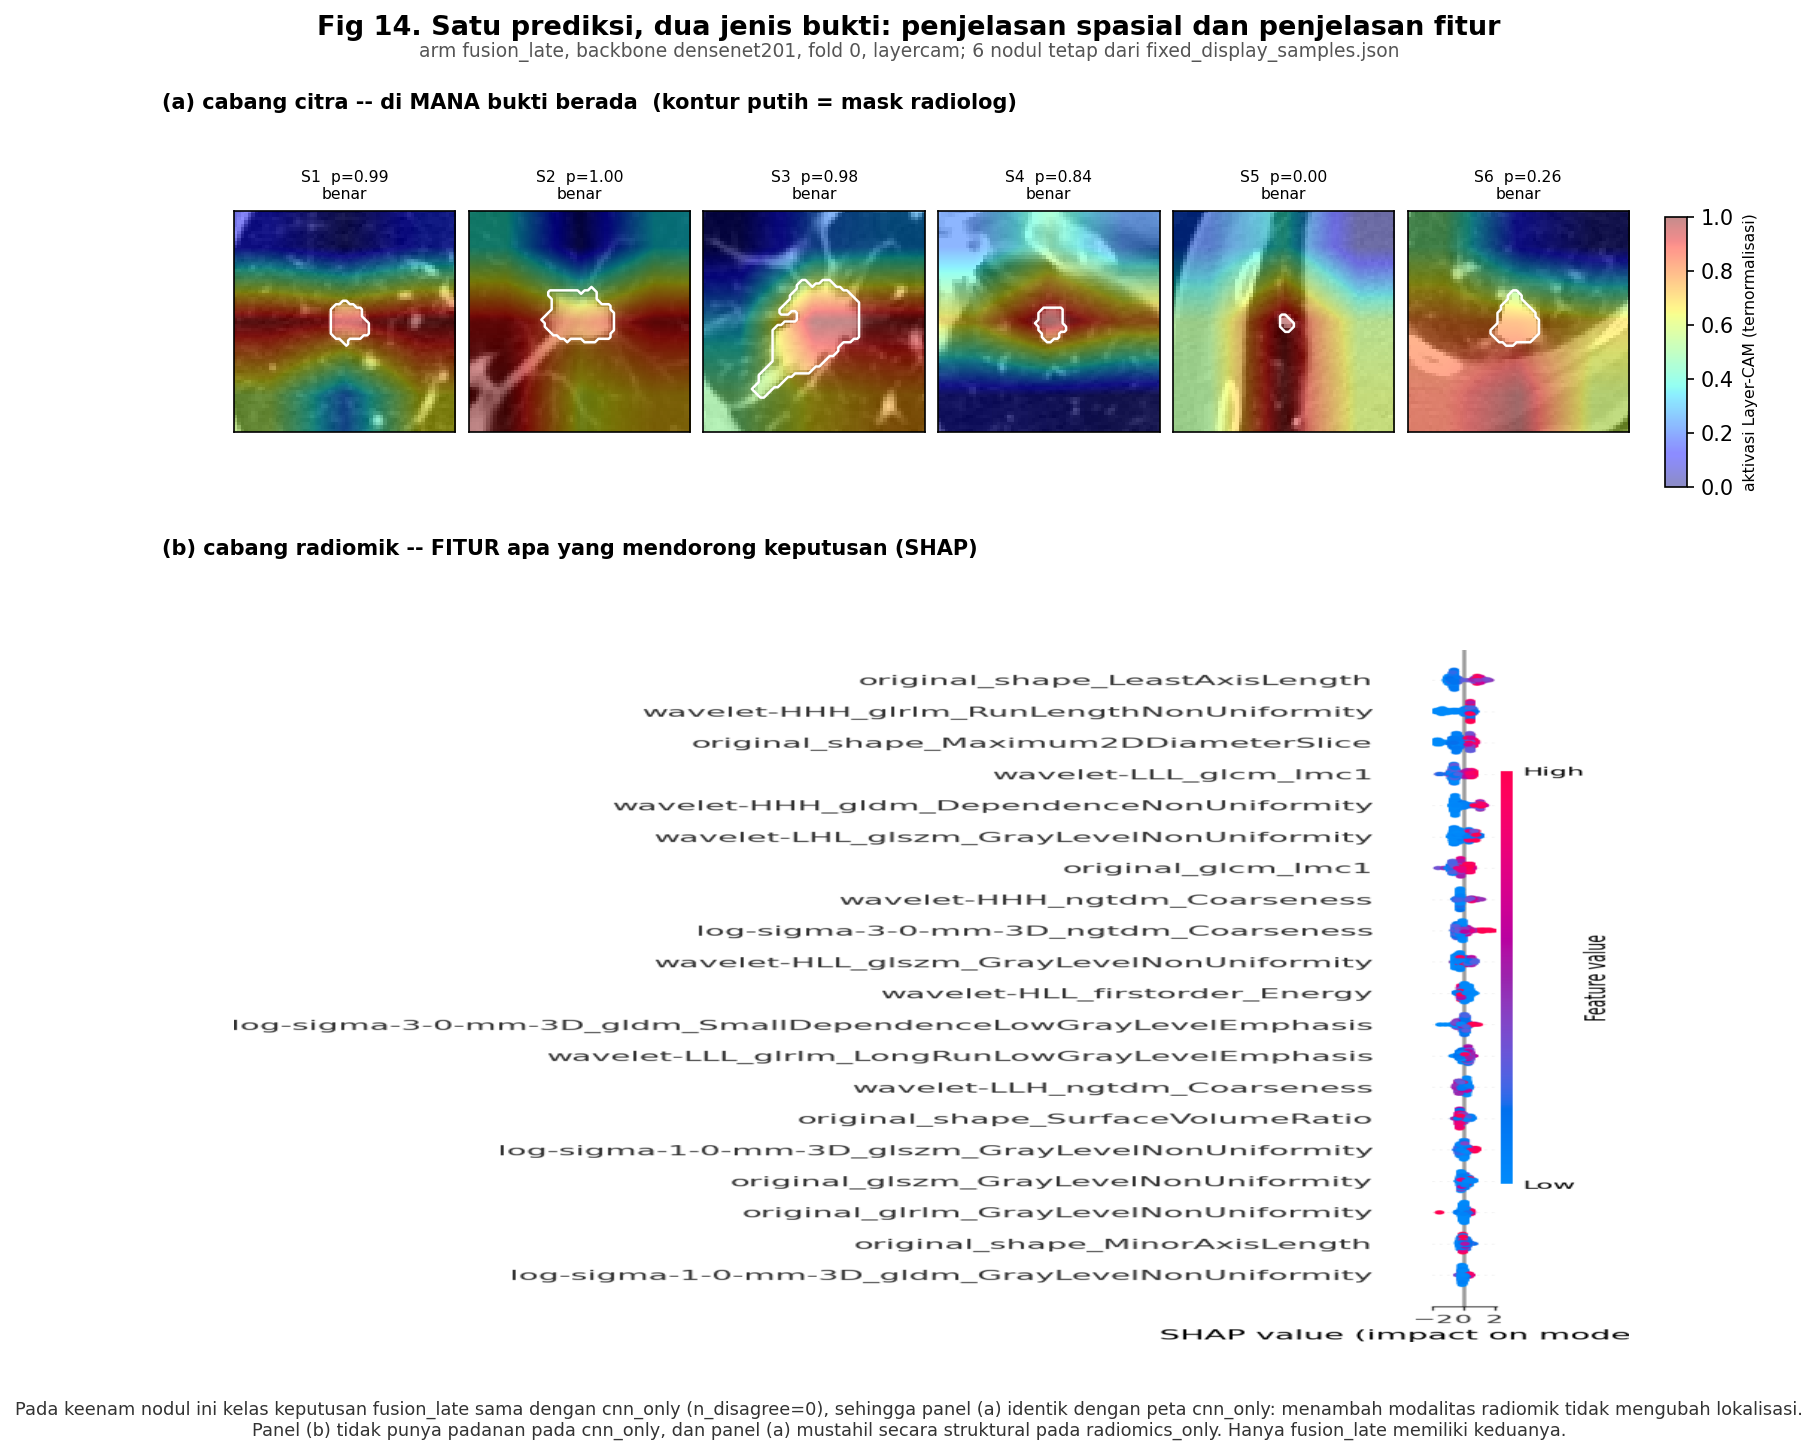
\includegraphics[width=\columnwidth]{fig14_spatial_and_feature.png}}
\caption{One prediction, two kinds of evidence, for the late-fusion arm on DenseNet201, fold 0. Top: Layer-CAM maps on the six fixed display nodules, with the radiologist mask outlined in white. Bottom: SHAP summary for the radiomics branch. Only the fused arm has both.}
\label{fig:fig14}
\end{figure}

\section{Discussion}
The result that survives every robustness check in this study is the weakest-sounding one: decision-level fusion beats the image modality alone, decisively and independently of checkpoint selection. That it holds under both regimes is structural rather than lucky, since both arms share the same CNN checkpoint. Claims comparing a selected arm against an unselected one, as the comparison against radiomics does, are the ones needing a stated regime, and we report both columns rather than the flattering one.

The equivalence result changes what the checkpoint regime means for this paper. Under a significance test the regime appears to decide the outcome, since two backbones cross $\alpha$ when the selection advantage is withdrawn. Under an equivalence test it decides nothing: all six comparisons clear the margin either way. Both readings come from one variance estimate on one set of probabilities, so the difference is not in the data but in the question. It is worth being explicit that this is the more demanding claim, not a softer one. Failing to reject equality is compatible with any true difference the sample is too small to see; rejecting the composite null of a difference of at least 0.02 excludes that possibility at the stated level, and would have failed had the differences been three times larger.

An honest reading of the accuracy result is that fusion earns no accuracy argument here, and we do not construct one. The literature is split on whether it should: several studies report clear fusion gains on lung nodules, and we do not claim they are wrong.\CITE{2--3 studi fusi yang melaporkan keunggulan} What we can say is bounded by this cohort and this fusion rule. The case for the fused arm rests instead on what it can be asked, which is the axis on which the single-modality arms are not merely worse but silent.

The explainability result deserves to be read as a positive finding rather than a shortfall. A fusion rule that averaged away the image branch's saliency, or that shifted attention off the nodule, would be a real cost of the added modality; the measurements show neither. The effect is bounded by construction: (\ref{eq:late}) leaves the image branch's weights untouched, so the map can change only where the fused decision differs from the CNN decision, which happens on 2 to 6 of 59 nodules. A difference of at most 0.05 in pointing accuracy, and exactly zero on the fixed display set, is the expected consequence of that structure, not an unexplained degradation.

What this buys clinically is a report that can be interrogated on two axes at once. A radiologist can ask where the model looked and receive a saliency map, and can ask which quantitative descriptors moved the decision and receive a ranked feature attribution, from the same prediction. Neither single-modality arm answers both questions, and on this cohort the fused arm answers them without paying for it in AUC.

\section{Limitations}
\label{sec:limits}
Statistical indistinguishability from radiomics-only is checkpoint-dependent on two of three backbones. Under the unselected checkpoint, DeLong rejects equality on ConvNeXt-Tiny ($p=0.0246$) and DenseNet121 ($p=0.0144$), with late fusion the lower arm in both. Equivalence within the 0.02 margin is not affected, and the two claims are compatible; but a reader who wants the stronger statement that no difference is detectable at all should attach either DenseNet201 or the selected regime to it. This does not touch the comparison against CNN-only, for the structural reason given above.

The equivalence margin is a judgement, not a measurement. A reader who considers 0.02 AUC clinically meaningful in this setting should read Table~\ref{tab:tost} as reporting intervals rather than verdicts; the intervals are given so that a different margin can be applied to them without re-running anything. We fixed $\delta$ before the analysis and did not revise it afterwards, but no procedure can make the choice itself objective.

The unselected-checkpoint analysis is a sensitivity check that bounds the effect of selection; it is not a nested cross-validation and does not remove selection from the training procedure itself.

Late fusion's pointing accuracy is nominally at or below CNN-only's on the 60-nodule set for every backbone. We report this alongside the fixed six-nodule set, where the two arms coincide exactly, rather than the latter alone. The explanation comparison also covers two arms, not five: the early- and intermediate-fusion arms are evaluated on AUC only, and no class-activation maps were computed for them, so this paper says nothing about what parameterised fusion does to localization.

The explainability metrics measure localization, not faithfulness. Pointing accuracy and its energy-based variant ask where a map lands relative to the annotated nodule; neither asks whether the map reflects the computation the model actually performed. A perturbation-based faithfulness measure would be the appropriate complement and is not reported here.\CITE{ROAD, Rong et al. ICML 2022} We treat this as an open item rather than a settled one.

There is no external validation. Every number in this paper comes from one dataset under one split, and reported performance on LIDC is known to move with sample-selection and label-truthing choices,\CITE{Baltatzis et al. 2021, pitfalls of sample selection} which is also why we make no comparison against AUC values reported by other LIDC studies: those are computed on different subsets and are not commensurable with ours. We note that LUNA16, the obvious candidate for an external cohort, is not a drop-in replacement, because its labels mark nodule versus non-nodule for detection rather than malignancy; external validation would require a cohort with malignancy ground truth, which we identify as the primary item of future work.

The explanations have not been evaluated by clinicians. A reader study would test whether the two explanation channels are usable rather than merely present, and a protocol for one accompanies this work, but no reader data were collected.

The radiomics feature selection uses a mutual-information filter followed by LASSO; an mRMR variant present in the codebase was never executed, and the reported numbers are those of the mutual-information path. SHAP and Layer-CAM attributions are reported on separate scales without a unifying model-agnostic metric, which we identify as an open methodological gap rather than a limitation specific to this study. Finally, the analysis covers three backbones selected in advance from a wider screen and one fixed fusion rule; no fusion architecture search was performed.

Reporting follows the CLAIM checklist for AI in medical imaging\CITE{CLAIM checklist, Mongan et al. 2020 / Tejani et al. 2024} and the TRIPOD+AI statement for prediction-model reporting.\CITE{TRIPOD+AI, Collins et al. 2024} The small-sample evaluation pitfalls catalogued for medical imaging machine learning\CITE{Varoquaux \& Cheplygina 2022} informed the frozen patient-level split, the pooled rather than averaged statistics, and the checkpoint-regime analysis.

\section{Conclusion}
On this cohort, decision-level fusion of a radiomics branch with a CNN branch significantly outperforms the CNN alone on every backbone tested and under both checkpoint regimes, and is equivalent to the stronger single modality within a pre-specified margin of 0.02 AUC on every backbone and under both regimes. That equivalence is established by a test whose null is a difference, not by a significance test that failed to find one. It preserves the image branch's spatial explanations at practically the same quality, differing only on the few nodules where the fused decision differs from the CNN decision, and it is the only arm supplying spatial and feature-level evidence for the same prediction. The contribution is therefore not a higher accuracy number but a model that matches the strongest single modality while remaining interrogable on both axes. A companion paper addresses backbone comparison, hyperparameter stability, and label granularity on the same dataset and split.

\section*{Acknowledgment}
The authors thank their supervisor and collaborators for guidance on this work.

\bibliographystyle{IEEEtran}
\bibliography{refs}

\end{document}
